% Options for packages loaded elsewhere
\PassOptionsToPackage{unicode}{hyperref}
\PassOptionsToPackage{hyphens}{url}
\PassOptionsToPackage{dvipsnames,svgnames*,x11names*}{xcolor}
%
\documentclass[
]{article}
\usepackage{amsmath,amssymb}
\usepackage{lmodern}
\usepackage{ifxetex,ifluatex}
\ifnum 0\ifxetex 1\fi\ifluatex 1\fi=0 % if pdftex
  \usepackage[T1]{fontenc}
  \usepackage[utf8]{inputenc}
  \usepackage{textcomp} % provide euro and other symbols
\else % if luatex or xetex
  \usepackage{unicode-math}
  \defaultfontfeatures{Scale=MatchLowercase}
  \defaultfontfeatures[\rmfamily]{Ligatures=TeX,Scale=1}
\fi
% Use upquote if available, for straight quotes in verbatim environments
\IfFileExists{upquote.sty}{\usepackage{upquote}}{}
\IfFileExists{microtype.sty}{% use microtype if available
  \usepackage[]{microtype}
  \UseMicrotypeSet[protrusion]{basicmath} % disable protrusion for tt fonts
}{}
\makeatletter
\@ifundefined{KOMAClassName}{% if non-KOMA class
  \IfFileExists{parskip.sty}{%
    \usepackage{parskip}
  }{% else
    \setlength{\parindent}{0pt}
    \setlength{\parskip}{6pt plus 2pt minus 1pt}}
}{% if KOMA class
  \KOMAoptions{parskip=half}}
\makeatother
\usepackage{xcolor}
\IfFileExists{xurl.sty}{\usepackage{xurl}}{} % add URL line breaks if available
\IfFileExists{bookmark.sty}{\usepackage{bookmark}}{\usepackage{hyperref}}
\hypersetup{
  pdftitle={Practical Work},
  pdfauthor={Rodrigo Arriaza, Alexander J Ohrt},
  colorlinks=true,
  linkcolor=Maroon,
  filecolor=Maroon,
  citecolor=Blue,
  urlcolor=blue,
  pdfcreator={LaTeX via pandoc}}
\urlstyle{same} % disable monospaced font for URLs
\usepackage[margin=1in]{geometry}
\usepackage{color}
\usepackage{fancyvrb}
\newcommand{\VerbBar}{|}
\newcommand{\VERB}{\Verb[commandchars=\\\{\}]}
\DefineVerbatimEnvironment{Highlighting}{Verbatim}{commandchars=\\\{\}}
% Add ',fontsize=\small' for more characters per line
\usepackage{framed}
\definecolor{shadecolor}{RGB}{248,248,248}
\newenvironment{Shaded}{\begin{snugshade}}{\end{snugshade}}
\newcommand{\AlertTok}[1]{\textcolor[rgb]{0.94,0.16,0.16}{#1}}
\newcommand{\AnnotationTok}[1]{\textcolor[rgb]{0.56,0.35,0.01}{\textbf{\textit{#1}}}}
\newcommand{\AttributeTok}[1]{\textcolor[rgb]{0.77,0.63,0.00}{#1}}
\newcommand{\BaseNTok}[1]{\textcolor[rgb]{0.00,0.00,0.81}{#1}}
\newcommand{\BuiltInTok}[1]{#1}
\newcommand{\CharTok}[1]{\textcolor[rgb]{0.31,0.60,0.02}{#1}}
\newcommand{\CommentTok}[1]{\textcolor[rgb]{0.56,0.35,0.01}{\textit{#1}}}
\newcommand{\CommentVarTok}[1]{\textcolor[rgb]{0.56,0.35,0.01}{\textbf{\textit{#1}}}}
\newcommand{\ConstantTok}[1]{\textcolor[rgb]{0.00,0.00,0.00}{#1}}
\newcommand{\ControlFlowTok}[1]{\textcolor[rgb]{0.13,0.29,0.53}{\textbf{#1}}}
\newcommand{\DataTypeTok}[1]{\textcolor[rgb]{0.13,0.29,0.53}{#1}}
\newcommand{\DecValTok}[1]{\textcolor[rgb]{0.00,0.00,0.81}{#1}}
\newcommand{\DocumentationTok}[1]{\textcolor[rgb]{0.56,0.35,0.01}{\textbf{\textit{#1}}}}
\newcommand{\ErrorTok}[1]{\textcolor[rgb]{0.64,0.00,0.00}{\textbf{#1}}}
\newcommand{\ExtensionTok}[1]{#1}
\newcommand{\FloatTok}[1]{\textcolor[rgb]{0.00,0.00,0.81}{#1}}
\newcommand{\FunctionTok}[1]{\textcolor[rgb]{0.00,0.00,0.00}{#1}}
\newcommand{\ImportTok}[1]{#1}
\newcommand{\InformationTok}[1]{\textcolor[rgb]{0.56,0.35,0.01}{\textbf{\textit{#1}}}}
\newcommand{\KeywordTok}[1]{\textcolor[rgb]{0.13,0.29,0.53}{\textbf{#1}}}
\newcommand{\NormalTok}[1]{#1}
\newcommand{\OperatorTok}[1]{\textcolor[rgb]{0.81,0.36,0.00}{\textbf{#1}}}
\newcommand{\OtherTok}[1]{\textcolor[rgb]{0.56,0.35,0.01}{#1}}
\newcommand{\PreprocessorTok}[1]{\textcolor[rgb]{0.56,0.35,0.01}{\textit{#1}}}
\newcommand{\RegionMarkerTok}[1]{#1}
\newcommand{\SpecialCharTok}[1]{\textcolor[rgb]{0.00,0.00,0.00}{#1}}
\newcommand{\SpecialStringTok}[1]{\textcolor[rgb]{0.31,0.60,0.02}{#1}}
\newcommand{\StringTok}[1]{\textcolor[rgb]{0.31,0.60,0.02}{#1}}
\newcommand{\VariableTok}[1]{\textcolor[rgb]{0.00,0.00,0.00}{#1}}
\newcommand{\VerbatimStringTok}[1]{\textcolor[rgb]{0.31,0.60,0.02}{#1}}
\newcommand{\WarningTok}[1]{\textcolor[rgb]{0.56,0.35,0.01}{\textbf{\textit{#1}}}}
\usepackage{longtable,booktabs,array}
\usepackage{calc} % for calculating minipage widths
% Correct order of tables after \paragraph or \subparagraph
\usepackage{etoolbox}
\makeatletter
\patchcmd\longtable{\par}{\if@noskipsec\mbox{}\fi\par}{}{}
\makeatother
% Allow footnotes in longtable head/foot
\IfFileExists{footnotehyper.sty}{\usepackage{footnotehyper}}{\usepackage{footnote}}
\makesavenoteenv{longtable}
\usepackage{graphicx}
\makeatletter
\def\maxwidth{\ifdim\Gin@nat@width>\linewidth\linewidth\else\Gin@nat@width\fi}
\def\maxheight{\ifdim\Gin@nat@height>\textheight\textheight\else\Gin@nat@height\fi}
\makeatother
% Scale images if necessary, so that they will not overflow the page
% margins by default, and it is still possible to overwrite the defaults
% using explicit options in \includegraphics[width, height, ...]{}
\setkeys{Gin}{width=\maxwidth,height=\maxheight,keepaspectratio}
% Set default figure placement to htbp
\makeatletter
\def\fps@figure{htbp}
\makeatother
\setlength{\emergencystretch}{3em} % prevent overfull lines
\providecommand{\tightlist}{%
  \setlength{\itemsep}{0pt}\setlength{\parskip}{0pt}}
\setcounter{secnumdepth}{-\maxdimen} % remove section numbering
\usepackage{booktabs}
\usepackage{longtable}
\usepackage{array}
\usepackage{multirow}
\usepackage{wrapfig}
\usepackage{float}
\usepackage{colortbl}
\usepackage{pdflscape}
\usepackage{tabu}
\usepackage{threeparttable}
\usepackage{threeparttablex}
\usepackage[normalem]{ulem}
\usepackage{makecell}
\usepackage{xcolor}
\ifluatex
  \usepackage{selnolig}  % disable illegal ligatures
\fi

\title{Practical Work}
\usepackage{etoolbox}
\makeatletter
\providecommand{\subtitle}[1]{% add subtitle to \maketitle
  \apptocmd{\@title}{\par {\large #1 \par}}{}{}
}
\makeatother
\subtitle{Lifetime Data Analysis}
\author{Rodrigo Arriaza, Alexander J Ohrt}
\date{15 desember, 2021}

\begin{document}
\maketitle

\hypertarget{introduction}{%
\section{Introduction}\label{introduction}}

We are given a data set on sexually transmitted diseases (STDs). This is data from a study about gonorrhea and chlamydia in 877 women. The objective with this practical work is to study possible risk factors for a reinfection with gonorrhea or chlamydia in women who have suffered one of both infections previously. The variables of interest are sociodemographic variables or those related to sexual practice. We have a lot of variables at our disposal, but have chosen to use the following, some for statistical reasons and some for medical reasons:

\begin{itemize}
\tightlist
\item
  Age: The age of the woman.
\item
  NumPartners: The number of partners during the last 30 days.
\item
  CondomUse: Use of condoms (1: always, 2: once in a while, 3: never)
\item
  YearsSchool: Years of schooling.
\item
  InitInfect: Initial infection (1: Gonorrhea, 2: Chlamydia, 3: both)
\item
  InvVagAtExam: Involvement vagina at exam (1: yes; 0: no).
\item
  DischargeExam: Discharge at exam (1: yes; 0: no)
\end{itemize}

The first three were chosen based on results from a \href{https://www.ncbi.nlm.nih.gov/pmc/articles/PMC1744639/}{study} on gonorrhea reinfection in heterosexual STD clinic attendees. The study concluded that increased reinfection risk (of gonorrhea) was associated with younger age and a greater number of recent sex partners, among other risk factors. Moreover, the authors concluded that any type of condom use was a risk factor for reinfection with gonorrhea in women.

Another \href{https://policylab.chop.edu/sites/default/files/pdf/publications/Preventing_Chlamydia_Gonorrhea_Reinfection_through_Increased_Use_of_EPT.pdf}{publication} reports that, on average, 14\% of women with clamydia and 12\% of women with gonorrhea get reinfected, with younger women at higher risk. Moreover, they state that many adolescents treated for infection of one of the two STDs are reinfected within three to six months, usually because of resumed sexual contact with an untreated partner. Thus, the marital status might be interesting to analyse. However, this is not added, because, the ages in the data set are low, which most likely means that the amount in each level of \texttt{MaritalStatus} is very skewed towards ``single''. This can be seen in the descriptive analysis below.

\href{https://www.ncbi.nlm.nih.gov/pmc/articles/PMC2094865/}{This meta-analysis} reports that the relationship between race, socioeconomic status (SES) and chlamydial infection is not clear. It concludes that SES was not associated with chlamydia infection, where they tested for several variables, where level of parent's education was one of them. Either way, we think it might be interesting to see if the years of schooling of the women (\texttt{YearsSchool}) have any impact on chlamydia reinfection and as is shown below it showed to be statistically significant during the exploratory analysis.

Moreover, we chose to use the initial infection (\texttt{InitInfect}) as an explanatory variable, because several of the studies above are only done on one of the two diseases, not on both at the same time. Because of this we wanted to investigate if the initial infection type is a risk factor and, if this is the case, if the risk differs based on which infection was suffered initially.

Naturally, the categorical variable which states if the woman is reinfected or not (\texttt{Reinfection}) will be used as a dependent variable in the analysis and the time until reinfection since the more time a subject is under study, the greater the risk of the event reoccurring.

\hypertarget{statistical-variable-selection}{%
\subsection{Statistical Variable Selection}\label{statistical-variable-selection}}

As noted, in addition to medical criteria for selecting variables, we have used the following statistical model to select variables based on statistical criteria. Shown below. RODRI: EXPLAIN!

REMOVE THIS AFTER: I made a list of things that can be used in the explanation:

\begin{itemize}
\tightlist
\item
  Despite the fact that the age of the woman is found to not be statistically significant in the method above, we have added it because of the mentioned studies (this is thus added based on medical criteria)
\end{itemize}

\begin{Shaded}
\begin{Highlighting}[]
\NormalTok{nb.model }\OtherTok{\textless{}{-}}\NormalTok{ MASS}\SpecialCharTok{::}\FunctionTok{glm.nb}\NormalTok{(Reinfection }\SpecialCharTok{\textasciitilde{}}\NormalTok{ Ethnicity }\SpecialCharTok{+}\NormalTok{ MaritalStatus }\SpecialCharTok{+}\NormalTok{ Age }\SpecialCharTok{+}\NormalTok{ YearsSchool }
          \SpecialCharTok{+}\NormalTok{ InitInfect }\SpecialCharTok{+}\NormalTok{ NumPartners }\SpecialCharTok{+}\NormalTok{OralSex12m }\SpecialCharTok{+}\NormalTok{ OralSex30d }\SpecialCharTok{+}\NormalTok{ RectalSex12m }
          \SpecialCharTok{+}\NormalTok{ RectalSex30d }\SpecialCharTok{+}\NormalTok{ AbPain }\SpecialCharTok{+}\NormalTok{ SignDischarge }\SpecialCharTok{+}\NormalTok{ SignDysuria }\SpecialCharTok{+}\NormalTok{ CondomUse }
          \SpecialCharTok{+}\NormalTok{ SignItch }\SpecialCharTok{+}\NormalTok{ SignLesion }\SpecialCharTok{+}\NormalTok{ SignRash }\SpecialCharTok{+}\NormalTok{ SignLymph }\SpecialCharTok{+}\NormalTok{ InvVagAtExam }
          \SpecialCharTok{+}\NormalTok{ DischargeExam }\SpecialCharTok{+}\NormalTok{ AbnormNodeExam }\SpecialCharTok{+} \FunctionTok{offset}\NormalTok{(}\FunctionTok{log}\NormalTok{(TimeUntilReinf)),}
              \AttributeTok{data=}\NormalTok{std\_data)}
\NormalTok{s }\OtherTok{\textless{}{-}} \FunctionTok{summary}\NormalTok{(nb.model)}
\NormalTok{k }\OtherTok{\textless{}{-}}\NormalTok{ knitr}\SpecialCharTok{::}\FunctionTok{kable}\NormalTok{(s}\SpecialCharTok{$}\NormalTok{coefficients, }\AttributeTok{caption =} \StringTok{\textquotesingle{}Statistical Significance of the Variables\textquotesingle{}}\NormalTok{)}
\NormalTok{kableExtra}\SpecialCharTok{::}\FunctionTok{row\_spec}\NormalTok{(k, }\FunctionTok{c}\NormalTok{(}\DecValTok{6}\NormalTok{,}\DecValTok{23}\NormalTok{,}\DecValTok{24}\NormalTok{), }\AttributeTok{color=}\StringTok{\textquotesingle{}white\textquotesingle{}}\NormalTok{, }\AttributeTok{background =} \StringTok{\textquotesingle{}blue\textquotesingle{}}\NormalTok{)}
\end{Highlighting}
\end{Shaded}

\begin{table}

\caption{\label{tab:variable-select}Statistical Significance of the Variables}
\centering
\begin{tabular}[t]{l|r|r|r|r}
\hline
  & Estimate & Std. Error & z value & Pr(>|z|)\\
\hline
(Intercept) & -4.4766626 & 0.6791361 & -6.5917022 & 0.0000000\\
\hline
EthnicityW & -0.0786114 & 0.1576156 & -0.4987540 & 0.6179527\\
\hline
MaritalStatusM & 0.1142920 & 0.4681139 & 0.2441542 & 0.8071114\\
\hline
MaritalStatusS & 0.5011754 & 0.3203698 & 1.5643657 & 0.1177317\\
\hline
Age & 0.0188481 & 0.0156143 & 1.2071011 & 0.2273932\\
\hline
\cellcolor{blue}{\textcolor{white}{YearsSchool}} & \cellcolor{blue}{\textcolor{white}{-0.1689015}} & \cellcolor{blue}{\textcolor{white}{0.0442657}} & \cellcolor{blue}{\textcolor{white}{-3.8156308}} & \cellcolor{blue}{\textcolor{white}{0.0001358}}\\
\hline
InitInfect2 & -0.3302518 & 0.1740868 & -1.8970524 & 0.0578210\\
\hline
InitInfect3 & -0.3318821 & 0.1755787 & -1.8902183 & 0.0587288\\
\hline
NumPartners & 0.1164568 & 0.0598373 & 1.9462257 & 0.0516276\\
\hline
OralSex12m1 & -0.3703474 & 0.2387666 & -1.5510855 & 0.1208812\\
\hline
OralSex30d1 & -0.3246975 & 0.2643311 & -1.2283739 & 0.2193066\\
\hline
RectalSex12m1 & 0.0669703 & 0.4881503 & 0.1371920 & 0.8908790\\
\hline
RectalSex30d1 & -0.1627456 & 0.6172379 & -0.2636675 & 0.7920361\\
\hline
AbPain1 & 0.2969178 & 0.1771403 & 1.6761734 & 0.0937042\\
\hline
SignDischarge1 & 0.1330009 & 0.1306664 & 1.0178660 & 0.3087416\\
\hline
SignDysuria1 & 0.1954606 & 0.1812469 & 1.0784219 & 0.2808455\\
\hline
CondomUse2 & -0.1553543 & 0.2725108 & -0.5700849 & 0.5686201\\
\hline
CondomUse3 & -0.4582270 & 0.2819913 & -1.6249684 & 0.1041693\\
\hline
SignItch1 & -0.2209724 & 0.1750560 & -1.2622958 & 0.2068424\\
\hline
SignLesion1 & -0.2541307 & 0.3787052 & -0.6710513 & 0.5021878\\
\hline
SignRash1 & -0.0638066 & 0.4592994 & -0.1389215 & 0.8895122\\
\hline
SignLymph1 & 0.2368538 & 0.5922357 & 0.3999317 & 0.6892069\\
\hline
\cellcolor{blue}{\textcolor{white}{InvVagAtExam1}} & \cellcolor{blue}{\textcolor{white}{0.5726933}} & \cellcolor{blue}{\textcolor{white}{0.2003764}} & \cellcolor{blue}{\textcolor{white}{2.8580874}} & \cellcolor{blue}{\textcolor{white}{0.0042620}}\\
\hline
\cellcolor{blue}{\textcolor{white}{DischargeExam1}} & \cellcolor{blue}{\textcolor{white}{-0.5805191}} & \cellcolor{blue}{\textcolor{white}{0.2691414}} & \cellcolor{blue}{\textcolor{white}{-2.1569301}} & \cellcolor{blue}{\textcolor{white}{0.0310111}}\\
\hline
AbnormNodeExam1 & 0.0801562 & 0.5157541 & 0.1554155 & 0.8764938\\
\hline
\end{tabular}
\end{table}

Finally, the vaginal involvement at exam (\texttt{InvVagAtExam}) and the discharge at exam (\texttt{DischargeExam}) are selected as variables in our analysis, since they are shown as statistically significant in the variable selection above.

\hypertarget{descriptive-analysis}{%
\section{Descriptive Analysis}\label{descriptive-analysis}}

In total, the data set contains 24 variables, but, as noted, we have selected only 7 of them in our analysis. Recall that the data set has 877 women. The percentage of right-censored data in the data set is 60.4, which is a relatively large part of the data set. The women where followed for 1529 days, then the study was stopped.

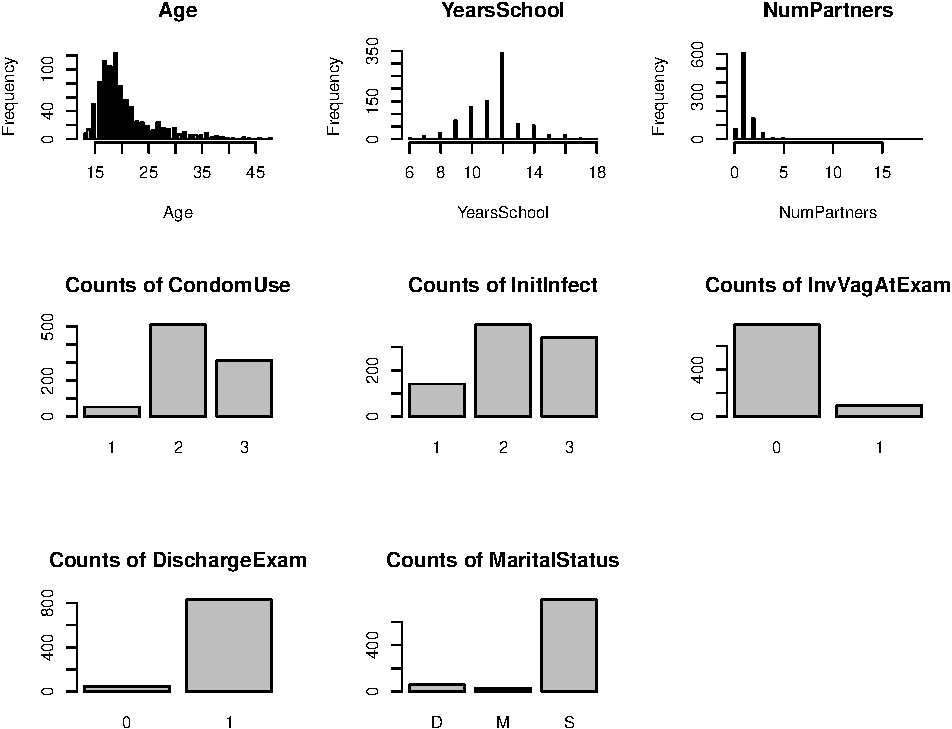
\includegraphics{practical_files/figure-latex/EDA-plots-1.pdf}
The three continuous variables we have chosen to use in the analysis are \texttt{Age}, \texttt{YearsSchool} and \texttt{NumPartners}. The correlations between the variables are shown in table \ref{tab:correlations}. Note that the correlation between \texttt{Age} and \texttt{YearsSchool} is 0.43, which means that they are somewhat correlated. This could be interesting to have in mind in the following.

\begin{table}

\caption{\label{tab:correlations}Corr. Between Continuous Variables}
\centering
\begin{tabular}[t]{l|c|c|c}
\hline
  & Age & YearsSchool & NumPartners\\
\hline
Age & 1.0000000 & 0.4316163 & 0.1348591\\
\hline
YearsSchool & 0.4316163 & 1.0000000 & 0.0155090\\
\hline
NumPartners & 0.1348591 & 0.0155090 & 1.0000000\\
\hline
\end{tabular}
\end{table}

\hypertarget{nonparametric-analysis}{%
\section{Nonparametric Analysis}\label{nonparametric-analysis}}

\hypertarget{survival-curve-estimation}{%
\subsection{Survival Curve Estimation}\label{survival-curve-estimation}}

The survival curve is estimated by means of Kaplan-Meier and plotted below. The curve below shows the general survival in the data set.

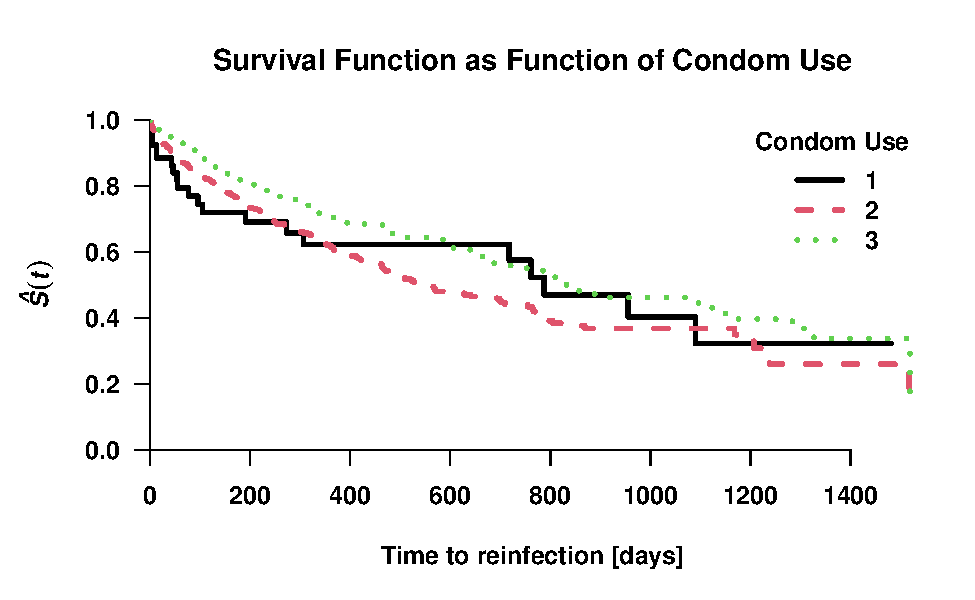
\includegraphics{practical_files/figure-latex/unnamed-chunk-1-1.pdf}

The median survival time is estimated to be 705 days.

\hypertarget{comparison-of-survival-curves}{%
\subsection{Comparison of Survival Curves}\label{comparison-of-survival-curves}}

Below, survival functions are compared by means of the nonparametric logrank test. Note that other types of tests also can be used (Fleming-Harrington family of tests), but we have only used the logrank test in this case. The general \(k\)-sample hypothesis that is tested is

\begin{equation*}
        H_0: S_1(t) = \ldots = S_k(t), \forall t \leq \tau \text{ vs. } H_1: \text{ some } S_i(t) \neq S_l(t), \text{ for some } t \leq \tau,
\end{equation*}

where \(\tau\) is the chosen limit of the time of examination and \(k\) varies depending on the levels of the explanatory variable we are testing. \textbf{What about tests on continuous variables, does this make sense as well?} The \(p\)-values from each of the tests are given in table \ref{tab:pvalues}. For instance, choosing a significance level of \(\alpha = 0.05\), we would conclude that reinfection depends on the level of \texttt{CondomUse}, \texttt{InitInfect} and \texttt{InvVagAtExam}, but that there is not enough evidence to conclude that reinfection depends on the level of \texttt{DischargeExam}.

\begin{table}

\caption{\label{tab:pvalues}p-values from logrank tests}
\centering
\begin{tabular}[t]{l|c|c|c|c}
\hline
  & CondomUse & InitInfect & InvVagAtExam & DischargeExam\\
\hline
p-values & 0.0132506 & 0.0145266 & 0.0068009 & 0.0558044\\
\hline
\end{tabular}
\end{table}

\hypertarget{fit-of-a-parametric-survival-model}{%
\section{Fit of a parametric survival model}\label{fit-of-a-parametric-survival-model}}

After trying to fit Weibull, log-logistic and lognormal log-linear models, we concluded that the Weibull model is best suited to our data.
\textbf{Should we have some interaction terms as well?}

\begin{verbatim}
#> 
#> Call:
#> survreg(formula = s2 ~ ., data = final.data, dist = "weibull")
#>                  Value Std. Error     z       p
#> (Intercept)     3.9516     0.6338  6.23 4.5e-10
#> Age             0.0101     0.0161  0.63 0.52912
#> NumPartners    -0.0139     0.0681 -0.20 0.83835
#> CondomUse2      0.0788     0.2995  0.26 0.79244
#> CondomUse3      0.4228     0.3106  1.36 0.17350
#> YearsSchool     0.1704     0.0487  3.50 0.00047
#> InitInfect2     0.5110     0.1907  2.68 0.00738
#> InitInfect3     0.3149     0.1915  1.64 0.10011
#> InvVagAtExam1  -0.5092     0.2212 -2.30 0.02133
#> DischargeExam1  0.4601     0.2894  1.59 0.11184
#> Log(scale)      0.2606     0.0445  5.85 4.9e-09
#> 
#> Scale= 1.3 
#> 
#> Weibull distribution
#> Loglik(model)= -2674.9   Loglik(intercept only)= -2697.1
#>  Chisq= 44.43 on 9 degrees of freedom, p= 1.2e-06 
#> Number of Newton-Raphson Iterations: 7 
#> n= 877
\end{verbatim}

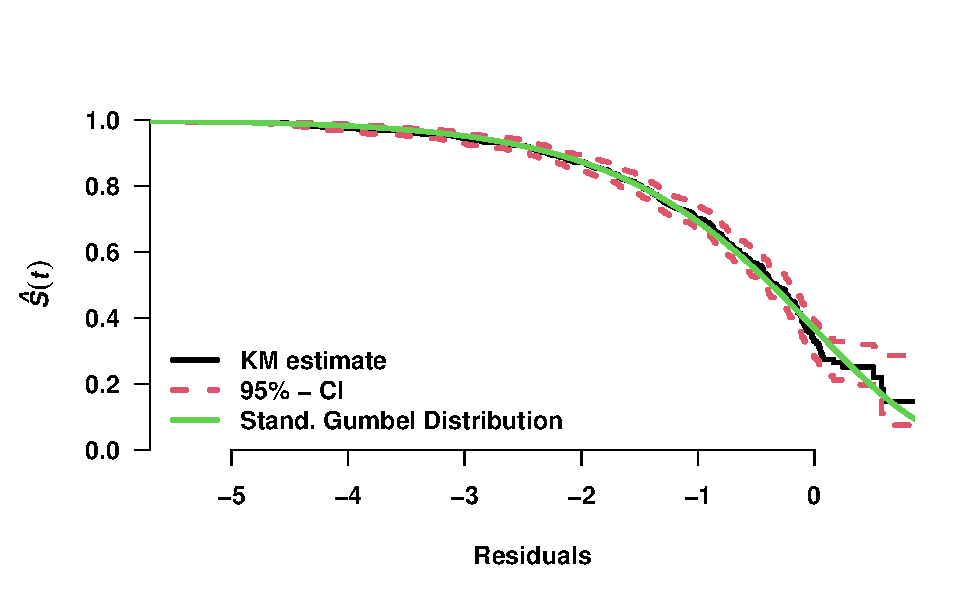
\includegraphics{practical_files/figure-latex/weibull-resids-1.pdf}

The standard Gumbel distribution seems to fit relatively nicely to the Kaplan-Meier estimate of the residuals, i.e.~it seems like a reasonable choice for the error term \(W\), which indicates that the Weibull is a reasonable model.

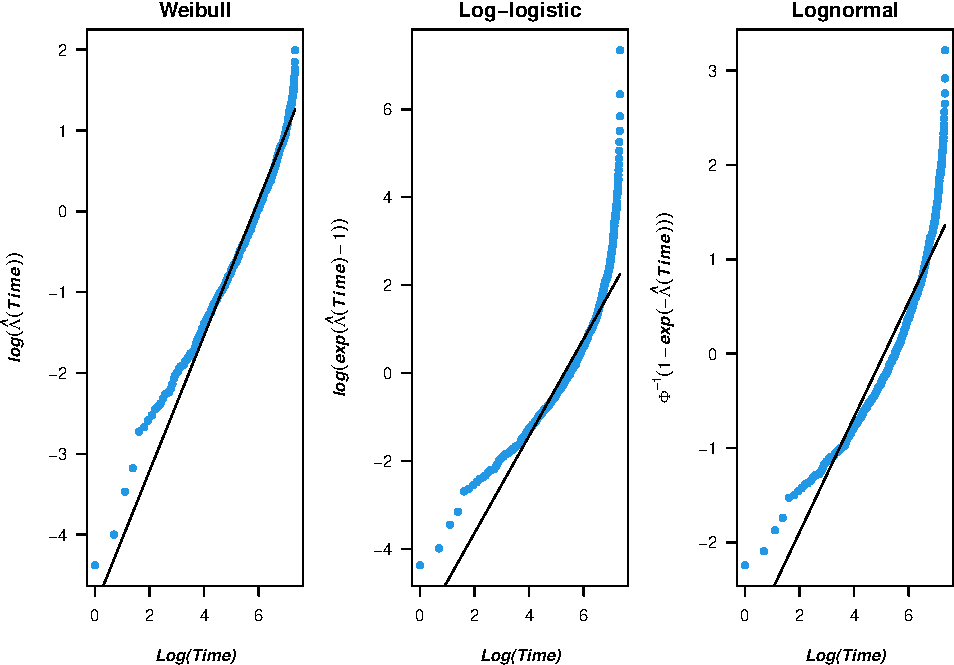
\includegraphics{practical_files/figure-latex/cumhaz-plot-1.pdf}

The probability plots above also show that the Weibull is the better parametric model for the data, because the log-logistic and lognormal models clearly do not fit the line in the tails.

How do we interpret this model fit? First of all, the model we have fit follows the expression

\[
Y = \ln(T) = \mu + \mathbf{\gamma}^T\mathbf{Z} + \sigma W,  
\]

where \(W \sim EV(0,1)\),

\[
\mathbf{\gamma}^T = (\gamma_{Age}, \gamma_{NumPartn.}, \gamma_{Cond.}, \gamma_{YSchool}, \gamma_{InitInf.}, \gamma_{InvVagAtExam.}, \gamma_{DischargeAtExam}),
\]

are the estimated parameters and

\[
\mathbf{Z}^T = (Age, NumPartn., Cond., YSchool, InitInf., InvVagAtExam., DischargeAtExam), 
\]

is the vector of values. Thus, each of the quantities \(\exp(\gamma_i)\) can be interpreted as the unitary change in time until reinfection (when the covariate \(i\) is continuous), or the change in time until reinfection when changing level (when the covariate \(i\) is categorical with different levels), when all the other explanatory variables are kept fixed.

In the Weibull model, the acceleration factor (AF) is calculated using the equation

\[
AF = \exp(-\hat{\gamma}_i)
\]
and the hazard ratio (HR) is calculated using the equation

\[
HR = \exp(-\hat{\gamma}_i/\hat{\sigma}).
\]
In this case, the model fit gives the scale \(\hat{\sigma} \approx\) 1.298. These values are calculated for each of the covariates below.

\begin{table}

\caption{\label{tab:unnamed-chunk-4}Parameter Estimates, AF and HR for each Parameter Estimate}
\centering
\begin{tabular}[t]{l|r|r|r}
\hline
  & Parameter.Estimate & AF & HR\\
\hline
(Intercept) & 3.9516047 & 0.0192238 & 0.0475893\\
\hline
Age & 0.0101018 & 0.9899491 & 0.9922457\\
\hline
NumPartners & -0.0138832 & 1.0139800 & 1.0107560\\
\hline
CondomUse2 & 0.0788112 & 0.9242144 & 0.9410747\\
\hline
CondomUse3 & 0.4227912 & 0.6552154 & 0.7219443\\
\hline
YearsSchool & 0.1704370 & 0.8432962 & 0.8769191\\
\hline
InitInfect2 & 0.5109972 & 0.5998971 & 0.6745026\\
\hline
InitInfect3 & 0.3149121 & 0.7298530 & 0.7845268\\
\hline
InvVagAtExam1 & -0.5091714 & 1.6639119 & 1.4804896\\
\hline
DischargeExam1 & 0.4601294 & 0.6312020 & 0.7014676\\
\hline
\end{tabular}
\end{table}

Consider an example using the covariate \texttt{CondomUse} when explaining the interpretation of the covariates in terms of the AF. From the table above it is apparent that the AF of \texttt{CondomUse3} versus \texttt{CondomUse1} is \(\approx\) 0.655. This means that the reinfection time for a person that never uses a condom is \(\approx\) 0.655 times the reinfection time for a person that always uses a condom \textbf{Not sure that this makes sense!? I think it makes sense with the coefficient value given from the model above, but does not make sense in real life, as this suggests that not using a condom is protective!} The interpretation in terms of the AF is similar when considering the other covariates, except for when considering the \texttt{Age} and \texttt{NumPartners}, which is not categorical \textbf{Perhaps it indeed makes sense to considering the Age in this way also, even though it is weird to treat the Age this way?}

The relative hazards (RH) can be calculated using the equation \ldots{}

\textbf{Is the relative hazards the same as the hazard ratio??}

\hypertarget{fit-of-a-semi-parametric-survival-model}{%
\section{Fit of a semi-parametric survival model}\label{fit-of-a-semi-parametric-survival-model}}

The proportional hazards model is below.

\begin{verbatim}
#> Call:
#> coxph(formula = s2 ~ ., data = final.data)
#> 
#>   n= 877, number of events= 347 
#> 
#>                     coef exp(coef)  se(coef)      z Pr(>|z|)    
#> Age            -0.007831  0.992200  0.012379 -0.633 0.526992    
#> NumPartners     0.011195  1.011258  0.052483  0.213 0.831083    
#> CondomUse2     -0.055195  0.946300  0.231217 -0.239 0.811326    
#> CondomUse3     -0.335706  0.714833  0.239486 -1.402 0.160981    
#> YearsSchool    -0.133564  0.874972  0.037403 -3.571 0.000356 ***
#> InitInfect2    -0.386802  0.679225  0.146484 -2.641 0.008277 ** 
#> InitInfect3    -0.235005  0.790567  0.147682 -1.591 0.111545    
#> InvVagAtExam1   0.401916  1.494686  0.170481  2.358 0.018396 *  
#> DischargeExam1 -0.367438  0.692506  0.223246 -1.646 0.099786 .  
#> ---
#> Signif. codes:  0 '***' 0.001 '**' 0.01 '*' 0.05 '.' 0.1 ' ' 1
#> 
#>                exp(coef) exp(-coef) lower .95 upper .95
#> Age               0.9922     1.0079    0.9684    1.0166
#> NumPartners       1.0113     0.9889    0.9124    1.1208
#> CondomUse2        0.9463     1.0567    0.6015    1.4888
#> CondomUse3        0.7148     1.3989    0.4470    1.1430
#> YearsSchool       0.8750     1.1429    0.8131    0.9415
#> InitInfect2       0.6792     1.4723    0.5097    0.9051
#> InitInfect3       0.7906     1.2649    0.5919    1.0560
#> InvVagAtExam1     1.4947     0.6690    1.0701    2.0877
#> DischargeExam1    0.6925     1.4440    0.4471    1.0726
#> 
#> Concordance= 0.602  (se = 0.017 )
#> Likelihood ratio test= 45.8  on 9 df,   p=7e-07
#> Wald test            = 46.94  on 9 df,   p=4e-07
#> Score (logrank) test = 47.21  on 9 df,   p=4e-07
\end{verbatim}

How do we interpret this model fit? First of all, the model we have fit follows the expression

\[
\lambda(t|\mathbf{Z}) =  \exp(\mathbf{\gamma}^T\mathbf{Z})\lambda_0(t),  
\]

where \(\gamma\) are the parameters in the model and \(\mathbf{Z}\) is the profile of the woman. Additionally, \(\lambda_0(t)\) is the hazard at time \(t\) for a woman with profile \(\mathbf{Z} = 0\), i.e.~a woman that always uses a condom, that was initially infected with (only) gonnorhea, that did not experience vaginal involvement at exam and did not experience discharge at exam. \textbf{Again: What do we do with the continuous covariates?}

\hypertarget{conclusions}{%
\section{Conclusions}\label{conclusions}}

Conclude on if some of the chosen explanatory variables are risk factors or protective factors for reinfection.

\end{document}
